%%% 特別研究報告書サンプル
\documentclass[dvipdfmx]{ampbt}

%%% クラスオプション:
%%% chapter:   \chapterコマンドを使用可能にする(jsbook (report) を使う).
%%% その他 jsclasses に指定可能なオプションが指定できます(そのまま渡される).

%%% 題目 %%%%%%%%%%%%%%%%%%%%%%%%%%%%%%%%%%%%%%%%%%%%%%%%%%%%%%%%%%%%%%%%%%%%%%%%
\title{境界積分方程式法による音場の}     % 題目1行目
      {数値解析と移動する受音点における}      % 題目2行目
      {リアルタイム可聴化について}                % 題目3行目
%%% 指導教員 %%%%%%%%%%%%%%%%%%%%%%%%%%%%%%%%%%%%%%%%%%%%%%%%%%%%%%%%%%%%%%%%%%%%
\supervisors{吉川仁}{准教授}    % 指導教員1人目 {氏名}{職名}
            {}{}    % 指導教員2人目 {氏名}{職名}
            {}{}                % 指導教員3人目 {氏名}{職名}
%%% 入学年月 %%%%%%%%%%%%%%%%%%%%%%%%%%%%%%%%%%%%%%%%%%%%%%%%%%%%%%%%%%%%%%%%%%%%
\entrancedate{26}{4}            % {年(平成)}{月}
%%% 著者氏名 %%%%%%%%%%%%%%%%%%%%%%%%%%%%%%%%%%%%%%%%%%%%%%%%%%%%%%%%%%%%%%%%%%%%
\author{石床}{竜一}             % {姓}{名}
%%% 提出日 %%%%%%%%%%%%%%%%%%%%%%%%%%%%%%%%%%%%%%%%%%%%%%%%%%%%%%%%%%%%%%%%%%%%%%
\submissiondate{30}{1}{26}      % {年(平成)}{月}{日}
%%% 背表紙の出力枚数 %%%%%%%%%%%%%%%%%%%%%%%%%%%%%%%%%%%%%%%%%%%%%%%%%%%%%%%%%%%%
\def\numberofspines{1}
%%% 摘要 %%%%%%%%%%%%%%%%%%%%%%%%%%%%%%%%%%%%%%%%%%%%%%%%%%%%%%%%%%%%%%%%%%%%%%%%
\abstract{%
  本研究では,一つの音源に対し、このモデルを用いて効率
  的に卒業論文を作成するためのアルゴリズムを開発した.また,このアルゴリズムを用
  いて,実際に本報告を作成した.その結果,従来の自分で執筆する方法に比べて,5000兆
  倍効率的に卒業論文を作成することが可能であることが確認された.
}
%%% パッケージの読み込みや自分用のマクロの定義 %%%%%%%%%%%%%%%%%%%%%%%%%%%%%%%%%%
\usepackage{amsmath,amssymb}
\usepackage{here}
\usepackage{bm}
\newcommand{\rme}{\mathrm{e}}

%%% 出力の制御 %%%%%%%%%%%%%%%%%%%%%%%%%%%%%%%%%%%%%%%%%%%%%%%%%%%%%%%%%%%%%%%%%%

%%% 本文を出力しない場合,次の行のコメントを外して下さい.
%% \outputbodyfalse

%%% 末尾に表紙,背表紙を出力しない場合,次の行のコメントを外して下さい.
%% \outputcoverfalse

%%% 末尾に提出用摘要を出力しない場合,次の行のコメントを外して下さい.
%% \outputabstractforsubmissionfalse

%%% ampbt.cls では表紙等の作成のために geometry パッケージを使用しているため,本文
%%% のレイアウトを変えるために \usepackage[...]{geometry} とすると Option clash が
%%% 発生します.何らかの理由で本文のレイアウトを変更したい場合は \geometry{...} を
%%% 使用して下さい.
%%% また,jsclasses を使用しているため,例えば 3cm を指定したい場合は 3truecm と書
%%% く必要があります.
%% \geometry{hmargin=3truecm,vmargin=2truecm}

\begin{document}
\ifoutputbody
%%% 中表紙,摘要,目次 %%%%%%%%%%%%%%%%%%%%%%%%%%%%%%%%%%%%%%%%%%%%%%%%%%%%%%%%%%
\makeinsidecover                % 中表紙
\makeabstract                   % 摘要
\maketoc                        % 目次
\setcounter{page}{1}            % 本文のページ番号を1から始める
%%% 本文 %%%%%%%%%%%%%%%%%%%%%%%%%%%%%%%%%%%%%%%%%%%%%%%%%%%%%%%%%%%%%%%%%%%%%%%%
\section{序論}
波動方程式は振動,音や光などの波動現象を記述するにあたって基本となる方程式であり,様々な手法を用いることで数値解析に
用いられてきた.また,波動方程式のような微分方程式に対し,取り扱う領域での境界に境界条件と呼ばれる付帯的な制限が与えられた
問題のことを境界値問題という.ところで近年,VR(バーチャルリアリティ)の研究が盛んになっており,博物館やアミューズメント施設,ゲームなどホビー要素の強いものから,
災害時の避難行動シミュレータ\cite{vrsaigai},歩行訓練機器への応用\cite{vrmedical}など実務的なものまでVRはいたるところに普及している.\par
本研究では波動方程式の解を数値計算し,VR空間上での観測を可能にするための基礎研究を目的とする.領域内に音源と壁が存在する空間での音圧の変化の計算は先行研究\cite{vrsound}では
道路交通の予測モデルであるASJ RTN-Model 2008を用いて計算していたが,本論文では領域の境界値を用いた波動方程式の解析手法である境界積分方程式を用いて領域内での音圧の計算を行った.
なお,ここで取り扱う境界値は点音源が発生する音圧から計算することとした.\par

本論文の構成は次の通りである.
% まず,第 2 章で Westervelt 方程式について説明し,さらに Westervelt 方程式の差分解法の定式化を示す.
% 第 3 章では第 2 章で導いた差分式を用いた数値計算結果を示す.
% 最後に第 4 章で結論を述べる.

\section{時間域境界積分方程式による音場解析}
\label{2章}
\subsection{対象とする問題}
\label{q}
ある閉じた三次元領域の外部$D$における,位置$\bm{x}$,時刻$t$での音圧を$u(\bm{x},t)$について
次の初期値境界値問題を考える.
\begin{align}
&\ddot{u}(\bm{x},t)-c^2 u_{,ii}(\bm{x},t)=0,\  \bm{x} \in D,\ t>0 \\
&u(\bm{x},0)=0,\  x \in D \\
&\dot{u}(\bm{x},0)=0,\  x \in D \\
&u(\bm{x},t)=\bar{u}(\bm{x},t),\  x\  \mbox{on} \ S_D,\ t>0 \\
&\frac{\partial{u}}{\partial{n}} (\bm{x},t)=\bar{q}(\bm{x},t),\  \bm{x}\  \mbox{on} \ S_N,\ t>0 \\
&u(\bm{x},t)=\bar{q}(\bm{x},t),\  \bm{x}\  \mbox{on} \ S_N,\ t>0
\end{align}
ここに$(\ )_{,i}$は$\dfrac{\partial{}}{\partial{x_i}}$,
$(\dot{\ })$は$\dfrac{\partial{}}{\partial{t}}$,
$\dfrac{\partial{}}{\partial{n}}$は法線微分で$n_i(\bm{x}) \dfrac{\partial{}}{\partial{x_i}}$,
$n(\bm{x})$は境界上の点$x$における領域の外向き単位法線ベクトル,
$S$は領域$D$の境界で$S=S_D \cup S_N$,
$c$は波速である.

\subsection{解の積分表現}
初期値境界値問題の解は,三次元波動方程式の基本解
\begin{align}
&\Gamma(\bm{x},t) = \displaystyle \frac{\delta(t-\dfrac{|x|}{c})}{4\pi|x|}
\end{align}
を用いて
\begin{equation}
  \label{eq:境界積分方程式}
u(\bm{x},t) = \int\!\!\!\int \Gamma(\bm{x}-y,t-s) \frac{\partial u}{\partial n}(y,s) - \int\!\!\!\int \frac{\partial \Gamma}{\partial n}(\bm{x}-y,t-s) \bar{u}(y,s) ds dS
\end{equation}
と表すことができる.
ここに$\delta(\bm{x})$はDiracのデルタ関数,
$t$は時刻,
$x$は領域内部の点,
$y$は境界上の点である.

\subsection{境界積分方程式の近似}
\label{kinji}
本研究では,受音点の各時刻での数値を境界積分方程式法を用いてリアルタイムに計算するが,%リアルタイムっていうやつの言葉とか
決められた時間内に特定の処理を終えなければならない制約ができる.そのため式(\ref{eq:境界積分方程式})を近似することを考える.\par
まず式(\ref{eq:境界積分方程式})第一項は基本解を代入して
\begin{align}
\int\!\!\!\int \dfrac{\delta(t-s-\dfrac{|x-y|}{c})}{4\pi|x-y|} \frac{\partial u}{\partial n}(y,s)dsdS
&= \int\!\!\!\int \dfrac{\delta(t-s-\dfrac{|x-y|}{c})}{4\pi|x-y|} \bar{q}(y,s)dsdS\\
&= \int\!\!\! \dfrac{1}{4\pi|x-y|} \bar{q}(y,t-\dfrac{|x-y|}{c})dS
\end{align}
となる.ここで,境界の面積分についての用いる.境界面を三角形で分割し,その各面要素を$S_j$とし,その面積を$S_j$とする.
面積分における各面積要素の積分値のために要する値が全て重心での値と等しいとし,面積の大きさ$S_j$との積をとることで
その面積要素の積分値の近似とする.この近似を用いるとき重心の値を$( )^g$と表記すれば,
\begin{align}
\int\!\!\! \dfrac{1}{4\pi|x-y|} \bar{q}(y,t-\dfrac{|x-y|}{c})dS &= \sum_j \int\!\!\! \dfrac{1}{4\pi|x-y_j|} \bar{q}(y_j,t-\dfrac{|x-y_j|}{c})dS_j \nonumber \\
&=\sum_j \dfrac{1}{4\pi|x-y_j^g|} \bar{q}(y_j^g,t-\dfrac{|x-y_j^g|}{c})S_j
\end{align}
\par
%%%%%%%%%%%%%%%%%%%%%%%%%%%%%%%一重層%%%%%%%%%%%%%%%%%%%%%%%%%%%%%%%%%%%%%%%%%%%%%%%%%%%%%%%%%%%%%%%%%%%%%%%%%%%%%%%%%%%%%%%%%%%%%%%%%%%%%%%%%%%%%%
次に,式(\ref{eq:境界積分方程式})第二項に基本解を代入したものを考える.
\begin{align}
\int\!\!\!\int \dfrac{\partial}{\partial n}\left( \dfrac{\delta(t-s-\dfrac{|x-y|}{c})}{4\pi|x-y|} \right) \bar{u}(y,s) ds dS
&= \int\!\!\!\int \dfrac{\partial}{\partial n}\left( \dfrac{\delta(t-s-\dfrac{|x-y|}{c})}{4\pi|x-y|} \right) \bar{u}(y,s) ds dS \nonumber \\
&= \int\!\!\!\int -n_i\dfrac{\partial}{\partial x_i}\left( \dfrac{\delta(t-s-\dfrac{|x-y|}{c})}{4\pi|x-y|} \right) \bar{u}(y,s) ds dS
\end{align}
式(\ref{eq:境界積分方程式})第一項と同様に三角形に境界面を分割すれば,
\begin{align}
\sum_j -n_i\dfrac{\partial}{\partial x_i}\int\!\!\!\int \left( \dfrac{\delta(t-s-\dfrac{|x-y_j|}{c})}{4\pi|x-y_j|} \right) \bar{u}(y_j,s) ds dS_j
\end{align}
ここで,時刻$t$を時間ステップ$n$と時間刻み幅$\Delta t$を用いて$t=n\Delta t$とする.ここで,境界量$\bar{u}(\bm{x},t)$の近似のため,
区分一定の空間内挿関$M^m(t)$を次のように定義する.
\begin{align}
  M^m(t) =
\begin{cases}
\; \dfrac{t}{\Delta t}-m+1,&\ (m-1)\Delta t \leq t \leq m\Delta t  \\
\; \dfrac{-t}{\Delta t}+m+1,&\ m\Delta t \leq t \leq (m+1)\Delta t  \\
\; 0, &\ \mbox{otherwise}
\end{cases}
\end{align}
これを用いると上式は
\begin{align}
\sum_j \sum_m -n_i\dfrac{\partial}{\partial x_i}\int\!\!\!\int_{(m-1)\Delta t }^{(m+1)\Delta t} \left( \dfrac{\delta(n\Delta t-s-\dfrac{|x-y_j|}{c})}{4\pi|x-y_j|} \right) \bar{u}(y_j,m\Delta t)M^m(s)dsdS_j
\end{align}
ここで$n\Delta t-s = \tau$とすれば,
\begin{align}
\sum_j \sum_m -n_i\dfrac{\partial}{\partial x_i}\int\!\!\!\int_{(n-m-1)\Delta t }^{(n-m+1)\Delta t} \left( \dfrac{\delta(\tau- \dfrac{|x-y_j|}{c})}{4\pi|x-y_j|} \right) \bar{u}(y_j,m\Delta t)M^m(n\Delta t - \tau)d\tau dS_j \nonumber \\
\label{eq:Ndounyuumae}
= \sum_j \sum_m -n_i\dfrac{\partial}{\partial x_i}\int\!\!\!\int_{(n-m-1)\Delta t }^{(n-m+1)\Delta t} \left( \dfrac{\delta(\tau- \dfrac{|x-y_j|}{c})}{4\pi|x-y_j|} \right) \bar{u}(y_j,m\Delta t)M^{n-m}(\tau)d\tau dS_j
\end{align}
となる.ここで,$N^m(t)$を次のように定義する.
\begin{align}
  N^m(t) =
\begin{cases}
\; -\dfrac{t}{\Delta t}+m,&\ 0 \leq t \leq m\Delta t  \\
\; 0, &\ \mbox{otherwise}
\end{cases}
\end{align}
$N^m(t)$を用いて式(\ref{eq:Ndounyuumae})を書き換えると,
\begin{align}
\label{eq:Ndounyuu}
&\sum_j \sum_m -n_i\dfrac{\partial}{\partial x_i}\int\!\!\!  \int_{0}^{(n-m+1)\Delta t} \left( \dfrac{\delta(\tau- \dfrac{|x-y_j|}{c})}{4\pi|x-y_j|} \right) \bar{u}(y_j,m\Delta t)N^{n-m+1}(\tau)d\tau dS_j \nonumber\\
&\hspace{2em} +2n_i\dfrac{\partial}{\partial x_i}\int\!\!\!  \int_{0}^{(n-m)\Delta t} \left( \dfrac{\delta(\tau- \dfrac{|x-y_j|}{c})}{4\pi|x-y_j|} \right) \bar{u}(y_j,m\Delta t)N^{n-m}(\tau)d\tau dS_j \nonumber \\
&\hspace{2em} -n_i\dfrac{\partial}{\partial x_i}\int\!\!\!  \int_{0}^{(n-m-1)\Delta t} \left( \dfrac{\delta(\tau- \dfrac{|x-y_j|}{c})}{4\pi|x-y_j|} \right) \bar{u}(y_j,m\Delta t)N^{n-m-1}(\tau)d\tau dS_j \nonumber\\
&= \sum_j \sum_m -n_i\dfrac{\partial}{\partial x_i}\int\!\!\! \dfrac{( (n-m+1)\Delta t - \dfrac{|x-y_j|}{c} )H((n-m+1)\Delta t - \dfrac{|x-y_j|}{c} )}{4\pi|x-y_j|\Delta t} \bar{u}(y_j,m\Delta t) dS_j \nonumber\\
&\hspace{2em} +2n_i\dfrac{\partial}{\partial x_i}\int\!\!\!  \dfrac{( (n-m)\Delta t- \dfrac{|x-y_j|)}{c} )H((n-m)\Delta t - \dfrac{|x-y_j|}{c} )}{4\pi|x-y_j|\Delta t}  \bar{u}(y_j,m\Delta t) dS_j \nonumber \\
&\hspace{2em} -n_i\dfrac{\partial}{\partial x_i}\int\!\!\!  \dfrac{( (n-m-1)\Delta t - \dfrac{|x-y_j|)}{c} )H((n-m-1)\Delta t - \dfrac{|x-y_j|}{c})}{4\pi|x-y_j|\Delta t}  \bar{u}(y_j,m\Delta t) dS_j
\end{align}
ここに,$H(\bm{x})$はHeavisideの階段関数である.式(\ref{eq:Ndounyuu})に対して,第一項に行ったように重心の値を代表値として近似を用いれば,
\begin{align}
\label{eq:ヘヴィサイド後}
&\sum_j \sum_m -n_i\dfrac{\partial}{\partial x_i} \left(\dfrac{( (n-m+1)\Delta t - \dfrac{|x-y^g_j|}{c} )H((n-m+1)\Delta t - \dfrac{|x-y^g_j|}{c} )}{4\pi|x-y^g_j|\Delta t} \bar{u}(y^g_j,m\Delta t) S_j \right) \nonumber\\
&\hspace{2em} +2n_i\dfrac{\partial}{\partial x_i}\left(\dfrac{( (n-m)\Delta t- \dfrac{|x-y^g_j|)}{c} )H((n-m)\Delta t - \dfrac{|x-y^g_j|}{c} )}{4\pi|x-y^g_j|\Delta t}  \bar{u}(y^g_j,m\Delta t) S_j \right) \nonumber \\
&\hspace{2em} -n_i\dfrac{\partial}{\partial x_i}\left(\dfrac{( (n-m-1)\Delta t - \dfrac{|x-y^g_j|)}{c} )H((n-m-1)\Delta t - \dfrac{|x-y^g_j|}{c})}{4\pi|x-y^g_j|\Delta t}  \bar{u}(y^g_j,m\Delta t) S_j \right) \nonumber \\
=&\sum_j \sum_m \dfrac{n_i(\bm{x}_i-y^g_i)}{4\pi \Delta t |x-y^g_j|^3}  \bar{u}(y^g_j,m\Delta t)(T^+H(T^+)-2TH(T)+T^-H(T^-) ) S_j  \nonumber\\
\end{align}
となる.ただし$T^+ =(n-m+1)\Delta t,\ T =(n-m)\Delta t,\ T^- =(n-m-1)\Delta t$である.
mについての値を陽に表記すると式(\ref{eq:ヘヴィサイド後})は
\begin{align}
\begin{cases}
  \label{eq:最後}
\; \displaystyle\sum_j \sum_m \dfrac{n_i(\bm{x}_i-y^g_i)}{4\pi \Delta t |x-y^g_j|^3}  \bar{u}(y^g_j,m\Delta t)(n-m+1)\Delta t S_j, &\dfrac{r}{c} < (n-m+1)\Delta t < \dfrac{r}{c}+\Delta t \\  \\
\; \displaystyle\sum_j \sum_m \dfrac{n_i(\bm{x}_i-y^g_i)}{4\pi \Delta t |x-y^g_j|^3}  \bar{u}(y^g_j,m\Delta t)(m-n+1)\Delta t S_j, &\dfrac{r}{c}+\Delta t < (n-m+1)\Delta t < \dfrac{r}{c}+2\Delta t\\  \\
\; 0, &\ \mbox{otherwise}
\end{cases}
\end{align}
となり,式(\ref{eq:最後})の上段,中段の不等式を満たす$m$をそれぞれ$m_1,m_2$とすれば,式(\ref{eq:境界積分方程式})第二項は
\begin{align}
\label{eq:最後の最後}
\displaystyle\sum_j \dfrac{n_i(\bm{x}_i-y^g_i)}{4\pi |x-y^g_j|^3} S_j \left\{  \bar{u}(y^g_j,m_1\Delta t)(n-m_1+1)
-2 \bar{u}(y^g_j,m_2\Delta t)(m_2-n+1)\right\}
\end{align}
となる.\par
%%%%%%%%%%%%%%%%%%%%%%%%%%%%%%%2重層%%%%%%%%%%%%%%%%%%%%%%%%%%%%%%%%%%%%%%%%%%%%%%%%%%%%%%%%%%%%%%%%%%%%%%%%%%%%%%%%%%%%%%%%%%%%%%%%%%%%%%%%%%%%%%
以上の結果をまとめると,式(\ref{eq:境界積分方程式})は
\begin{align}
\label{eq:境界積分方程式の変形後}
u(\bm{x},t) = &\sum_j  \dfrac{1}{4\pi|x-y_j^g|} \bar{q}(y_j^g,t-\dfrac{|x-y_j^g|}{c}) \nonumber\\
 &+ \dfrac{n_i(\bm{x}_i-y^g_i)}{4\pi |x-y^g_j|^3} S_j \left\{  -\bar{u}(y^g_j,m_1\Delta t)(n-m_1+1)
 +2 \bar{u}(y^g_j,m_2\Delta t)(m_2-n+1)\right\}
\end{align}
となる.以降この式を用いて,境界内の各時間ステップ毎の音圧を数値計算した.




\section{近似手法の評価}

\subsection{境界値の取得}
\label{境界値の取得}
境界積分方程式には境界条件が必要であるが,本論文では以下のように与えた.以下数値の単位はメートル[m]とする.
まず,壁を中心(0.5,0.5,0.5)で,x,y,z軸に各面が平行であるものを考えた.
つぎに,壁の内部に音源が存在するものとし,その音源(source)の位置$x^s$と音源の発生させる音圧$f(t)$を以下のようにする.
\begin{align}
x^s &= (0.25,0.25,0.25)\\
\label{ef:f(t)}
f(t) &= 1-cos(\dfrac{2 \pi}{\lambda}t)
\end{align}
ここに,\ $\lambda = 1.25 \times 10^{-3}$[m]\ である.
また,境界$S$について,第\ref{kinji}節で行った三角形分割を行い,その三角形の重心を代表点とすれば,
各三角形面$S_j$での境界値は次のように与えることができる.
\begin{align}
\bar{u}(\bm{x}_j,t) &= \dfrac{1-cos\dfrac{2 \pi}{\lambda}(t-\dfrac{r}{c})}{4\pi|x^g_j-x^s|} \\
\bar{q}(\bm{x}_j,t) &= \dfrac{\partial \bar{u}}{\partial n} \nonumber \\
               &= \dfrac{-1}{4\pi|x^g_j-x^s|^2}((\bm{x}_j)_i-x^s_i)n_i \left\{ \dfrac{1-cos\dfrac{2 \pi}{\lambda}(t-\dfrac{r}{c})}{r} + \dfrac{2\pi}{\lambda c} sin\dfrac{2\pi}{\lambda}(t-\dfrac{r}{c})  \right\}
\end{align}
これを境界値の$\bar{u}(\bm{x},t),\bar{q}(\bm{x},t)$とする.

\subsection{解析的手法と近似手法との比較}
第\ref{2章}章で行った近似を用い,領域内での受音点での数値計算結果をここで述べる.まず,入力として与えた$f(t)$を図\ref{fig:ft}に図示する
\begin{figure}[htbp]
  \begin{center}
    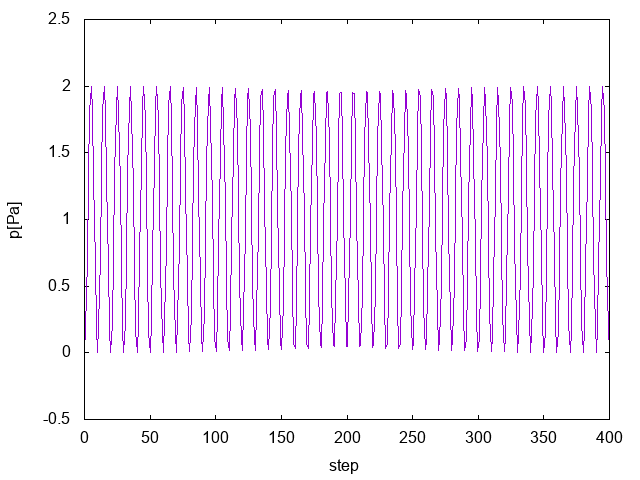
\includegraphics[clip,width=9.0cm]{./png/ft.png}
    \caption{音源$f(t)$}
    \label{fig:ft}
  \end{center}
\end{figure}\\
ここに,x軸は時刻$t=n\Delta t$としたときの$n$を表し,y軸は時刻$f(n\Delta t)$の音圧を表す.\par
$f(t)$と第\ref{境界値の取得}節で解析的に求めた境界値を用い,領域内点で,受音点が観測する音圧を計算させた.
その結果と,音源からの距離減衰と距離遅延を加味した,次に解析的に定義される波形$u_{ans}(\bm{x},t)$と比較する.
\begin{align}
u_{ans}(\bm{x},t) &= \dfrac{f(t-\dfrac{|x-x^s|}{c})}{4\pi |x-x^s|}
\end{align}
以下は図\ref{fig:original_u}は$u_{ans}(\bm{x},t)$,図\ref{fig:naiten_u}は近似手法によるであり図\ref{fig:mix_u}は図\ref{fig:original_u}と図\ref{fig:naiten_u}を重ね合わせたものでである.,観測点はともに$x^s &= (-0.5,0.5,0.5)$である.
%こたえ
\begin{figure}[H]
  \begin{center}
    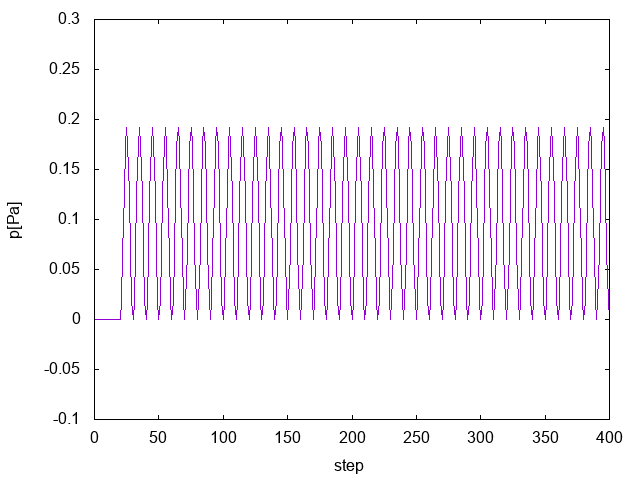
\includegraphics[clip,width=10.0cm]{./png/original_u.png}
    \caption{$u_{ans}(t)$}
    \label{fig:original_u}
  \end{center}
\end{figure}\\
%内点の図
\begin{figure}[H]
  \begin{center}
    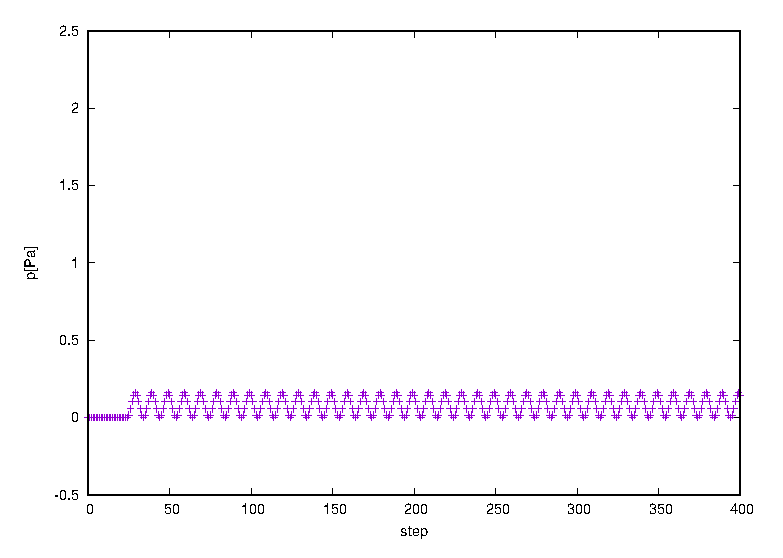
\includegraphics[clip,width=10.0cm]{./eps/original_u.eps}
    \caption{内点計算による$u(\bm{x},t)$}
    \label{fig:naiten_u}
  \end{center}
\end{figure}\\
%重ねたやつ
\begin{figure}[H]
  \begin{center}
    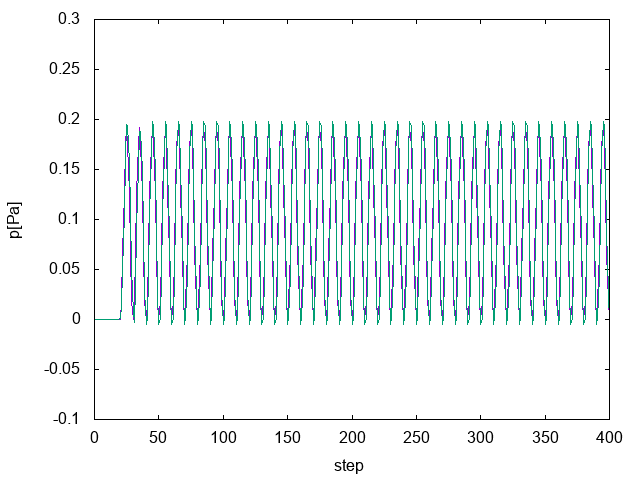
\includegraphics[clip,width=10.0cm]{./png/mix_u.png}
    \caption{図\ref{fig:original_u}と図\ref{fig:naiten_u}を重ねたもの}
    \label{fig:mix_u}
  \end{center}
\end{figure}\\

さらに,数値的な比較をいかに行う.ここでの評価基準は2ノルムで,2ノルムは
\begin{align}
\sum_m \dfrac{\{u_{ans}(\bm{x},m\Delta t)-u(\bm{x},m\Delta t)\}^2}{ \{u_{ans}(\bm{x},m\Delta t)\}^2 }
\end{align}
である.この評価を用いた場合,計算結果は$2.4 \times 10^{-3}$となった.ここに,総ステップ数は$f_s=8000$つまり1秒分のデータである.

\section{リアルタイム可聴化のためのシステム概要}
\subsection{リアルタイム可聴化の定義}
第\ref{q}節で定式化した問題を第\ref{kinji}節で示した近似を用いて計算するが,ここでリアルタイムの定義について記す.
実用上のリアルタイムとは実時間的,即時的という言葉である.音の場合,サンプリングレートを$f_s$[Hz]とすれば,1秒間を$f_s$個のデータで構成することになる.
本論文では,$1/f_s$秒毎に内点計算を行うことで,時刻$t$に対し$tf_s$個の計算を終了させることをリアルタイム計算とし,作成したデータから即時的にデータから音へ変換することで,
可聴化することをリアルタイム可聴化と定義する.

\subsection{実行環境と開発システムについて}
リアルタイム可聴化を行う前に,移動する受音点の状況をわかりやすくするため音源,受音点,壁を可視化した.
可視化には'Uity Version 2017 .3.0f3 Personal'を用いた.
\subsection{プログラム}
がんばったところとか




\clearpage
%%% 謝辞 %%%%%%%%%%%%%%%%%%%%%%%%%%%%%%%%%%%%%%%%%%%%%%%%%%%%%%%%%%%%%%%%%%%%%%%%
\acknowledgment
本研究に取り組むにあたって助言をいただいた吉川仁准教授,計算幾科学コース新田泰大氏に深く感謝
する.

%%% 参考文献 %%%%%%%%%%%%%%%%%%%%%%%%%%%%%%%%%%%%%%%%%%%%%%%%%%%%%%%%%%%%%%%%%%%%
\addcontentsline{toc}{section}{\refname} % 目次に参考文献を追加する.
                                         % chapter使用時は削除すること.
\begin{thebibliography}{10}
\bibitem{vrsaigai}
目黒公郎, et al. バーチャルリアリティの避難行動シミュレータへの応用. 土木学会論文集, 1997, 556: 197-207.
\bibitem{vrmedical}
藤江正克, et al. バーチャルリアリティを活用した歩行訓練機器. BME, 1998, 12.8: 29-37.
\bibitem{vrsound}
田近伸二; 樫山和男; 志村正幸. VR 技術を用いた対話型道路交通騒音評価システムの構築. 応用力学論文集, 土木学会, 2010, 13: 231-240.
\end{thebibliography}
%%% BibTeX 等を用いる場合は,上の thebibliography 環境を消してここに該当コードを
%%% 挿入すること.
%% \bibliographystyle{...}
%% \bibliography{...}

%%% 付録 %%%%%%%%%%%%%%%%%%%%%%%%%%%%%%%%%%%%%%%%%%%%%%%%%%%%%%%%%%%%%%%%%%%%%%%%
%%% 付録は不要ならば削除してよい.
\appendix

\section{意味のない付録}
これは意味のない付録です.これは意味のない引用です\cite{polya1945}.

\begin{table}[htbp]
  \caption{これは意味のない表です.}
  \centering
  \begin{tabular}{c|cc}
      &  A  &  B \\
    \hline
    C &  70 & 80 \\
    D & 100 &  0
  \end{tabular}
\end{table}

%%% 本文ここまで %%%%%%%%%%%%%%%%%%%%%%%%%%%%%%%%%%%%%%%%%%%%%%%%%%%%%%%%%%%%%%%%
\fi
\ifoutputcover
\cleardoublepage
%%% 表紙,背表紙,提出用摘要 %%%%%%%%%%%%%%%%%%%%%%%%%%%%%%%%%%%%%%%%%%%%%%%%%%%%
\makecover                      % 表紙
\makespine[\numberofspines]     % 背表紙
\fi
\ifoutputabstractforsubmission
\makeabstractforsubmission      % 提出用摘要
\fi
\end{document}
